\section{PROBLEM FORMULATION}\label{sec:problem}

The pre-capture phase starts with the chaser some ten meters away from a freely tumbling, noncooperative target and ends when the chaser holds a capture pose in front of the target docking port. This section states the dynamics and the prediction model available to the chaser, the capture geometry and the safety constraints, and the resulting optimization problem, and it closes with an analysis of the features that shape the methods of Sections~\ref{sec:framework} and~\ref{sec:ecc}.

\subsection{Dynamics and Prediction Model}\label{sec:dynamics}

Three right-handed frames are used (Fig.~\ref{fig:scene}): the Earth-centered inertial frame $\FI$, the target body frame $\FT$ aligned with the principal axes of the target, and the chaser body frame $\FC$, whose $x$-axis, with unit vector $\vect{e}_{\mathrm{C}}$, is the camera boresight. The configuration of each spacecraft is described on the Lie group $\SE$, which represents attitude and position jointly and without singularities \cite{yang2025taes,gong2026ast}. The pose is $\bg=(\bR,\bp)\in\SE$, where $\bR\in\SO$ maps the body frame to $\FI$ and $\bp\in\R^{3}$ is the inertial position, and the body twist is $\bxi=[\bw^{\T},\bnu^{\T}]^{\T}$ with angular velocity $\bw$ and translational velocity $\bnu$. Following \cite{yang2025taes}, the motion of each rigid body obeys
\begin{align}
\dot{\bg} &= \bg\,\bxi^{\wedge}, \label{eq:kin}\\
\bJ\dot{\bw} &= -\bw\times\bJ\bw+\bG_{\mathrm{g}}+\bG, \label{eq:rot}\\
m\dot{\bnu} &= -m\,\bw\times\bnu+\bff_{\mathrm{g}}+\bff, \label{eq:trans}
\end{align}
where $m$ and $\bJ$ are the mass and the inertia matrix and $(\bG,\bff)$ is the control wrench in the body frame. With $\bp_{\mathrm{b}}=\bR^{\T}\bp$, $p=\norm{\bp}$, and $\bM=\tfrac12\mathrm{tr}(\bJ)\bI_{3}-\bJ$, the gravitational wrench consists of the gravity-gradient torque and the central force with its second-order mass-moment correction and the $J_{2}$ perturbation \cite{yang2025taes,tian2024taes},
\begin{align}
\bG_{\mathrm{g}} &= \frac{3\mu}{p^{5}}\,\bp_{\mathrm{b}}\times\bJ\bp_{\mathrm{b}},\label{eq:tg}\\
\bff_{\mathrm{g}} &= -\frac{\mu m}{p^{3}}\bp_{\mathrm{b}}-\frac{3\mu}{p^{5}}\bM\bp_{\mathrm{b}}+\frac{15\mu\,\bp_{\mathrm{b}}^{\T}\bM\bp_{\mathrm{b}}}{2p^{7}}\bp_{\mathrm{b}}+\bR^{\T}\bff_{J_{2}},\label{eq:fg}
\end{align}
where $\mu$ is the gravitational parameter of the Earth and $\bff_{J_{2}}$ is the $J_{2}$ force in $\FI$. The subscripts $\mathrm{T}$ and $\mathrm{C}$ refer to the target and the chaser. The relative pose and twist are $\bg_{\mathrm{r}}=\bg_{\mathrm{T}}^{-1}\bg_{\mathrm{C}}$ and $\bxi_{\mathrm{r}}=\bxi_{\mathrm{C}}-\mathrm{Ad}_{\bg_{\mathrm{r}}^{-1}}\bxi_{\mathrm{T}}$; their exponential coordinates form the relative state used by the near-field controller. The relative position is $\brho=\bp_{\mathrm{C}}-\bp_{\mathrm{T}}$ with range $\rho=\norm{\brho}$ and velocity $\bv=\dot{\brho}$, and $\brhoT=\bR_{\mathrm{T}}^{\T}\brho$ is the same position expressed in $\FT$. The joint state of the two spacecraft is denoted by $X=(\bg_{\mathrm{T}},\bxi_{\mathrm{T}},\bg_{\mathrm{C}},\bxi_{\mathrm{C}})$.

The control wrench is held constant over each control period $\Delta t$ and is bounded per axis by $\norm{\bff}_{\infty}\le\fmax$ and $\norm{\bG}_{\infty}\le\Gmax$. The propellant used up to time $t$ is measured by the velocity increment
\begin{equation}\label{eq:dv}
\Delta v(t)=\int_{0}^{t}\frac{\norm{\bff_{\mathrm{C}}(t')}}{\mC}\,\dd t'.
\end{equation}

\begin{assumption}\label{ass:info}
The relative state and the attitude and angular velocity of the target are measured; the inertia of the target is unknown to the chaser.
\end{assumption}

Under Assumption~\ref{ass:info}, every prediction of the target attitude used for decision and planning holds the current angular velocity constant,
\begin{equation}\label{eq:pred}
\hat{\bR}_{\mathrm{T}}(t+\tau)=\bR_{\mathrm{T}}(t)\exp\bigl(\tau\,\bw_{\mathrm{T}}(t)^{\times}\bigr),\qquad \tau\ge0,
\end{equation}
which is the torque-free motion of a body with isotropic inertia. The prediction rotates the target about the inertial spin axis $\bs=\bR_{\mathrm{T}}\bw_{\mathrm{T}}/\Omega$ at the spin rate $\Omega=\norm{\bw_{\mathrm{T}}}$ with spin period $\Ts=2\pi/\Omega$. The translational model used for planning is the double integrator
\begin{equation}\label{eq:di}
\ddot{\brho}=\bff/\mC
\end{equation}
in inertial axes, which neglects the differential gravity over the short ranges considered. Only the dynamics \eqref{eq:kin}--\eqref{eq:fg} use the true inertia.

\begin{figure}[t]
\centering
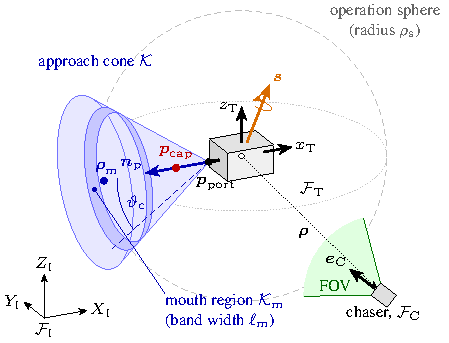
\includegraphics{figures/fig_scene.pdf}
\caption{Pre-capture scene (target enlarged for legibility). The port and the capture point are fixed in $\FT$ and rotate with the target about the spin axis $\bs$; the approach cone $\Kset$ of half-angle $\vartheta_{\mathrm{c}}$ opens along the port axis $\bnp$, and the operation sphere of radius $\rhos$ surrounds the target.}
\label{fig:scene}
\end{figure}

\subsection{Capture Geometry and Constraints}\label{sec:constraints}

The docking port $\bpport$, its approach axis $\bnp$, and the capture point $\bpcap$ are fixed in $\FT$, with $\bpport$ and $\bpcap$ on the port axis. The port direction in $\FI$ is $\bn=\bR_{\mathrm{T}}\bnp$; since the target tumbles, the capture point moves in $\FI$ and the chaser must meet a rotating interface rather than a fixed point. With the axial coordinate $\ell(\vect{u})=\bnp^{\T}(\vect{u}-\bpport)$, the approach cone is
\begin{equation}\label{eq:cone}
\begin{aligned}
\Kset=\bigl\{\vect{u}\in\R^{3}:\ &\ell(\vect{u})\ge\ell_{\min},\\
&\norm{\vect{u}-\bpport-\ell(\vect{u})\bnp}\le\ell(\vect{u})\tan\vartheta_{\mathrm{c}}\bigr\}.
\end{aligned}
\end{equation}
The operation sphere is the ball of radius $\rhos$ about the target center, and the mouth region $\Km=\{\brhoT\in\Kset:\rho<\rhos+\ell_{\mathrm{m}}\}$ extends it by a band of width $\ell_{\mathrm{m}}$ inside the cone. Approach speeds are limited by the braking envelope $\vb(\ell)$, a piecewise-linear inner approximation of the constant-deceleration profile $\sqrt{v_{\mathrm{f}}^{2}+\fmax\ell/\mC}$; every segment is a chord of this concave profile, so that $\vb$ is nowhere looser than it.

The safe set $\Sset$ is the set of joint states $X$ that satisfy the constraints of Table~\ref{tab:constraints}, where $d_{\mathrm{clr}}$ is the clearance between the envelope sphere of the chaser and the target body including its grapple rod, the radial closing speed $-\dot\rho$ is measured in $\FI$, and the speeds in $\Km$ are measured relative to the rotating target. The classification follows \cite{tian2024taes,xu2026ast}; actuator saturation is a limit, not a constraint violation. The capture set $\Xcap$ contains the joint states with $\brhoT\in\Kset$ whose position, attitude, velocity, and angular-velocity errors with respect to the capture pose at $\bpcap$ are within given tolerances, and the capture time $\tc$ is the first instant at which the state has remained in $\Xcap$ for a holding time $T_{\mathrm{c}}$.

\begin{table}
\caption{Safety Constraints}
\label{tab:constraints}
\tablefont
\begin{tabular*}{\columnwidth}{@{\extracolsep{\fill}}>{\raggedright\arraybackslash}p{4.9pc}>{\raggedright\arraybackslash}p{3.3pc}>{\raggedright\arraybackslash}p{9.4pc}@{}}
\hline
Constraint & Region & Condition\\
\hline
Collision & All & $d_{\mathrm{clr}}\ge0$\\
Sphere or corridor & All & $\rho\ge\rhos$ or $\brhoT\in\Kset$\\
Field of view & All & $\angle\bigl(\bR_{\mathrm{C}}\vect{e}_{\mathrm{C}},\,\bR_{\mathrm{T}}\bpport-\brho\bigr)\le\vartheta_{\mathrm{fov}}$\\
Radial braking & $\brhoT\notin\Km$ & $-\dot\rho\le\vb(\rho-\rhos)$\\
Relative speed & $\brhoT\in\Km$ & $\norm{\dot{\brho}_{\mathrm{T}}}\le\bar v_{\mathrm{m}}$\\
Axial braking & $\brhoT\in\Km$ & $-\bnp^{\T}\dot{\brho}_{\mathrm{T}}\le\vb\bigl(\bnp^{\T}(\brhoT-\bpcap)\bigr)$\\
Range & All & $\rho\le\bar\rho$\\
\hline
\end{tabular*}
\end{table}

\subsection{Problem Statement and Analysis}\label{sec:mission}

Each task carries mission parameters drawn from a mission distribution: a deadline $\Td$, a velocity-increment budget $\Bmax$, and weights $c_{\mathrm{t}}$ and $c_{\mathrm{f}}$ that price time and propellant. The pre-capture problem is to find a feedback law, from the measurements of Assumption~\ref{ass:info} to the control wrench of the chaser, that solves the following problem.

\noindent\textit{Problem~1:}
\begin{equation}\label{eq:problem}
\begin{aligned}
\min\ \ & \E\bigl[c_{\mathrm{t}}\tc+c_{\mathrm{f}}\Delta v(\tc)\bigr]\\
\text{s.t.}\ \ & \eqref{eq:kin}\text{--}\eqref{eq:fg},\ \ \norm{\bff}_{\infty}\le\fmax,\ \ \norm{\bG}_{\infty}\le\Gmax,\\
& X(t)\in\Sset,\ \ t\in[0,\tc],\\
& \tc\le\Td,\qquad \Delta v(\tc)\le\Bmax,
\end{aligned}
\end{equation}
where the expectation is taken over the target state, the initial relative state, and the mission parameters. The requirements of \eqref{eq:problem} cannot be met for every realization; Section~\ref{sec:mdp} therefore replaces them with terminal penalties when the problem is cast as a decision process.

Problem~1 has a temporal structure that a short-horizon constrained optimization does not capture. By \eqref{eq:pred}, the port direction $\bn$ sweeps periodically about $\bs$, and a safe entry along the port axis is possible only while $\bn$ points toward the chaser. These passes recur with period $\Ts$, and an entry must begin by the latest admissible time $\te=\Td-\Tr$, where the reserve $\Tr$ leaves time for the final approach to the capture point. With $\taup(t)$ the time to the center of the next pass, the opportunity margin
\begin{equation}\label{eq:eta}
\eta(t)=\frac{\te-t-\taup(t)}{\Ts}
\end{equation}
measures, in spin periods, the time that remains after the next pass (Fig.~\ref{fig:timeline}). Under \eqref{eq:pred} with the line of sight held fixed, exactly $\lfloor\eta\rfloor+1$ pass centers precede $\te$ when $\eta\ge0$; for $0\le\eta<1$ the next pass is the last one, and missing it leaves no further pass before $\te$. Opportunities are scarce when $\eta<1$.

\begin{figure}[t]
\centering
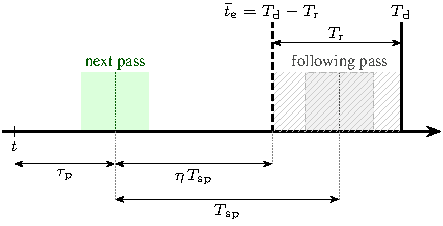
\includegraphics{figures/fig_timeline.pdf}
\caption{Opportunity structure of Problem~1. Passes of the port recur with the spin period $\Ts$; an entry must begin by $\te=\Td-\Tr$. The opportunity margin $\eta$ in \eqref{eq:eta} counts the spin periods left after the next pass; in the case shown, $\eta<1$ and the next pass is the last one.}
\label{fig:timeline}
\end{figure}

Five features follow. 1)~The port sweeps periodically, so the time at which an entry is possible is decided by the rotation of the target. 2)~Whether a pass is usable depends on how closely the line of sight approaches the sweep of the port, and when it occurs depends on the phase of the port. 3)~An entry plan can fail during execution, and abandoning the pass costs about one spin period. 4)~Whether an intent can be converted into an entry is resolved by the execution layer on a time scale of seconds and is not visible in the outcome until much later. 5)~When $\eta<1$, neighboring decisions can lead to capture and timeout, respectively. Features 1--3 raise the question of how to steer the chaser, with a low-dimensional decision, so that passes become usable and correctly timed; Section~\ref{sec:framework} answers it with rotation-synchronized window guidance. Features 4 and 5 raise the question of how a learned decision layer, whose decisions take effect only through the rules of a constrained executor, can account for opportunities that only the executor resolves; Section~\ref{sec:ecc} answers it with execution-feedback closed-loop coordination.
